% Options for packages loaded elsewhere
\PassOptionsToPackage{unicode}{hyperref}
\PassOptionsToPackage{hyphens}{url}
%
\documentclass[
]{article}
\usepackage{amsmath,amssymb}
\usepackage{lmodern}
\usepackage{iftex}
\ifPDFTeX
  \usepackage[T1]{fontenc}
  \usepackage[utf8]{inputenc}
  \usepackage{textcomp} % provide euro and other symbols
\else % if luatex or xetex
  \usepackage{unicode-math}
  \defaultfontfeatures{Scale=MatchLowercase}
  \defaultfontfeatures[\rmfamily]{Ligatures=TeX,Scale=1}
\fi
% Use upquote if available, for straight quotes in verbatim environments
\IfFileExists{upquote.sty}{\usepackage{upquote}}{}
\IfFileExists{microtype.sty}{% use microtype if available
  \usepackage[]{microtype}
  \UseMicrotypeSet[protrusion]{basicmath} % disable protrusion for tt fonts
}{}
\makeatletter
\@ifundefined{KOMAClassName}{% if non-KOMA class
  \IfFileExists{parskip.sty}{%
    \usepackage{parskip}
  }{% else
    \setlength{\parindent}{0pt}
    \setlength{\parskip}{6pt plus 2pt minus 1pt}}
}{% if KOMA class
  \KOMAoptions{parskip=half}}
\makeatother
\usepackage{xcolor}
\usepackage[margin=1in]{geometry}
\usepackage{graphicx}
\makeatletter
\def\maxwidth{\ifdim\Gin@nat@width>\linewidth\linewidth\else\Gin@nat@width\fi}
\def\maxheight{\ifdim\Gin@nat@height>\textheight\textheight\else\Gin@nat@height\fi}
\makeatother
% Scale images if necessary, so that they will not overflow the page
% margins by default, and it is still possible to overwrite the defaults
% using explicit options in \includegraphics[width, height, ...]{}
\setkeys{Gin}{width=\maxwidth,height=\maxheight,keepaspectratio}
% Set default figure placement to htbp
\makeatletter
\def\fps@figure{htbp}
\makeatother
\setlength{\emergencystretch}{3em} % prevent overfull lines
\providecommand{\tightlist}{%
  \setlength{\itemsep}{0pt}\setlength{\parskip}{0pt}}
\setcounter{secnumdepth}{-\maxdimen} % remove section numbering
\usepackage{hyperref}
\hypersetup{colorlinks=false, linktoc=all, linkcolor=red}
\usepackage{placeins}
\usepackage{caption}
\usepackage{fancyhdr}
\usepackage{lipsum}
\pagestyle{fancy}
\fancyhead[R]{\thepage}
\usepackage{amsmath}
\usepackage{algpseudocode}
\usepackage{algorithm}
\ifLuaTeX
  \usepackage{selnolig}  % disable illegal ligatures
\fi
\IfFileExists{bookmark.sty}{\usepackage{bookmark}}{\usepackage{hyperref}}
\IfFileExists{xurl.sty}{\usepackage{xurl}}{} % add URL line breaks if available
\urlstyle{same} % disable monospaced font for URLs
\hypersetup{
  pdftitle={P8106 Final Project},
  pdfauthor={Wenjia Zhu, Ruihan Zhang, Jasmine Niu},
  hidelinks,
  pdfcreator={LaTeX via pandoc}}

\title{P8106 Final Project}
\author{Wenjia Zhu, Ruihan Zhang, Jasmine Niu}
\date{May 10, 2023}

\begin{document}
\maketitle

{
\setcounter{tocdepth}{2}
\tableofcontents
}
\newpage

\hypertarget{background}{%
\section{Background}\label{background}}

To better understand the factors that predict recovery time from
COVID-19 illness, a study was designed to combine three existing cohort
studies that have been tracking participants for several years. The
study collects recovery information through questionnaires and medical
records and leverages existing data on personal characteristics before
the pandemic.

\hypertarget{introduction}{%
\section{Introduction}\label{introduction}}

The aim of this research is to develop a prediction model for recovery
time from COVID-19 by merging three cohort studies that have been
following participants for several years. Recovery information will be
gathered through questionnaires and medical records, and personal
characteristics data from before the pandemic will be utilized. The
ultimate goal is to develop a prediction model for recovery time and
identify important risk factors for a long recovery time.

\hypertarget{data-and-exploratory-analysis}{%
\section{Data and Exploratory
Analysis}\label{data-and-exploratory-analysis}}

This study employs the recovery.RData file, which comprises a dataset of
10,000 participants. The dataset contains a variable for recovery time
from COVID-19 (in days) along with 14 predictor variables, including
demographic features, personal characteristics, vital measurements, and
disease status. The predictors consist of both continuous and
categorical variables. The study used two merged random samples of 2000
participants, which were obtained from the seed set to 2631 and 2855
respectively, to create the final dataset. The training dataset contains
80\% of the sample and, the test dataset contains the remaining 20\%.

\begin{center}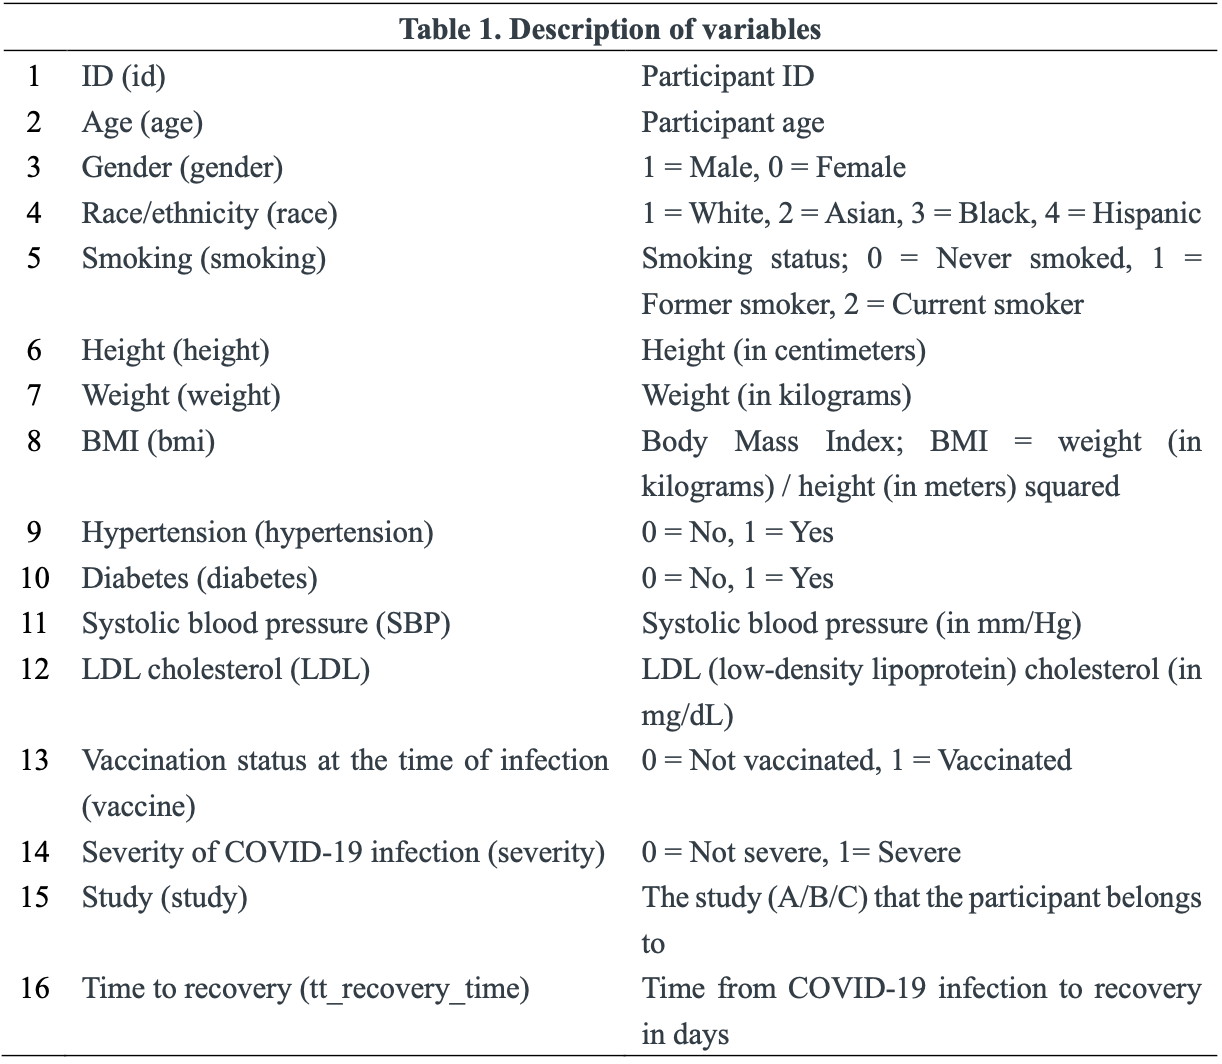
\includegraphics[width=0.9\linewidth,height=0.7\textheight]{./first} \end{center}

\begin{center}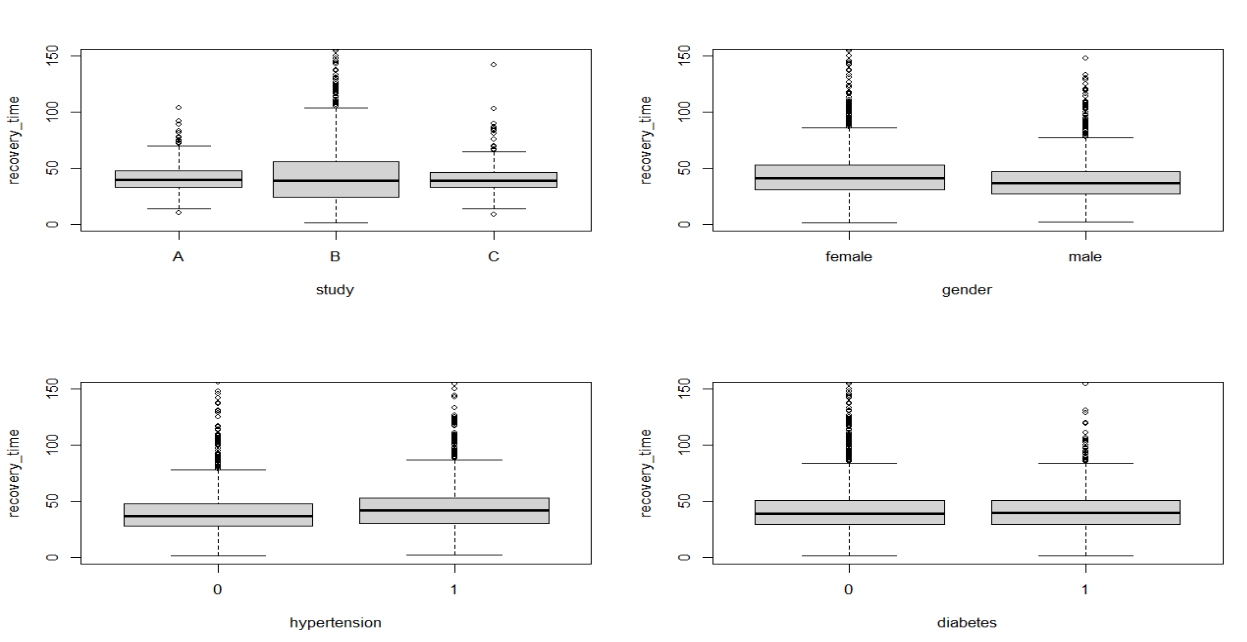
\includegraphics[width=0.9\linewidth,height=0.7\textheight]{primary_analysis_plot/Explanatory analysis and visualization_boxplot_1} \end{center}
\begin{center}
Figure 1. the relationship between continuous predictors(sbp, ldl, age, weight, height and bmi) and recovery time
\end{center}

Five lattice plots have been used to visualize the relationship between
continuous predictors(sbp, ldl, age, weight, height and bmi) and
recovery time. There is almost no relationship between sbp and recovery
time, between age and recovery time, and between ldl and recovery time.
There is a positive relationship between height and recovery time, and
between weight and recovery time. There is a negative relationship
between bmi and recovery time.

\begin{center}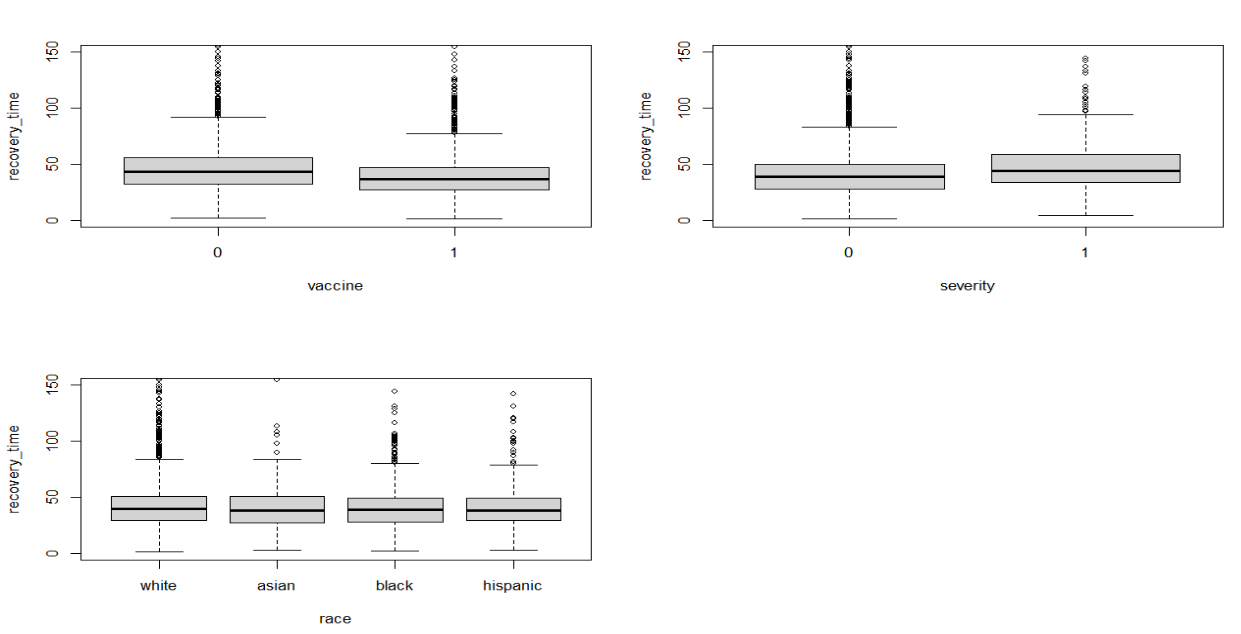
\includegraphics[width=0.9\linewidth,height=0.7\textheight]{primary_analysis_plot/Explanatory analysis and visualization_boxplot_2} \end{center}

\begin{center}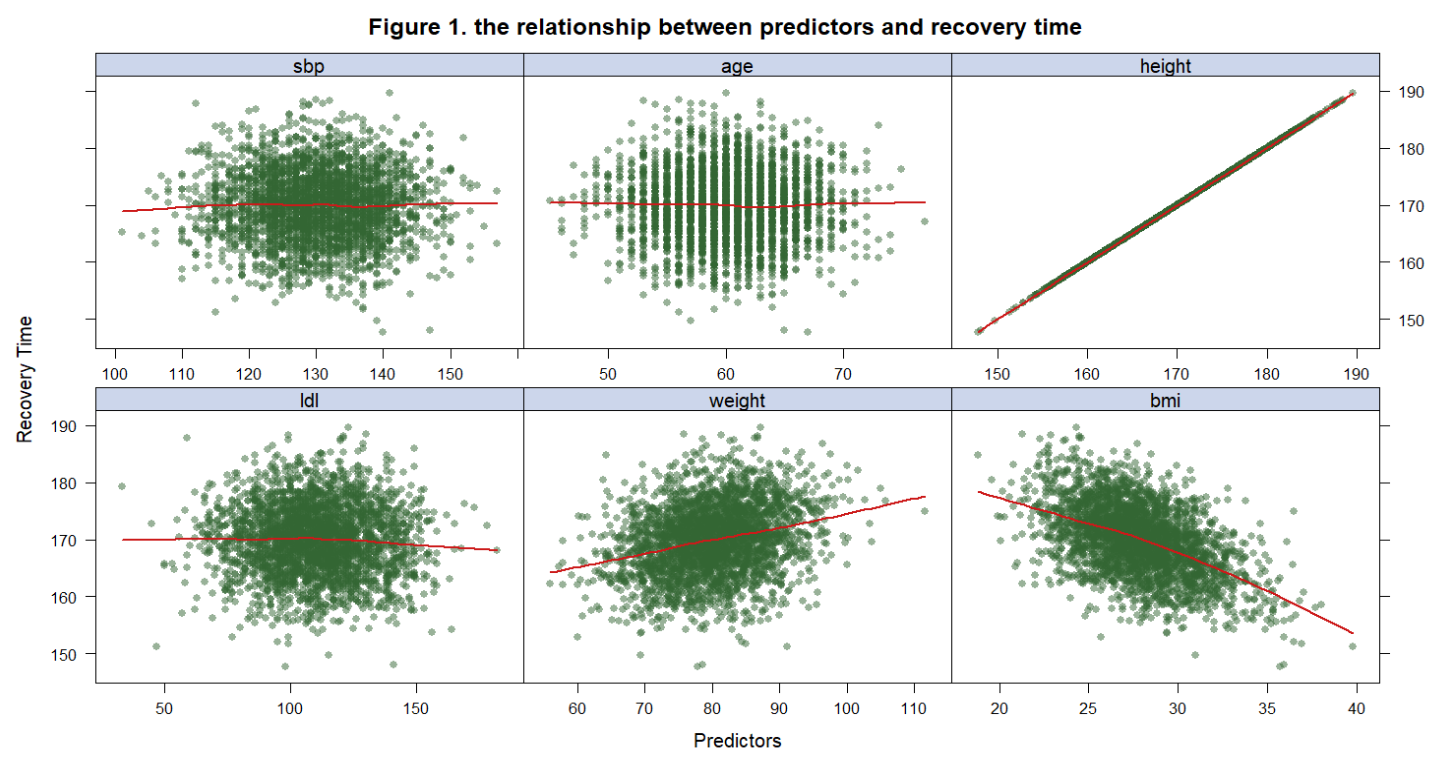
\includegraphics[width=0.9\linewidth,height=0.7\textheight]{primary_analysis_plot/Explanatory analysis and visualization_scatterplot} \end{center}
\begin{center}
Figure 2. the relationship between categorical predictors(study, hypertension, gender, diabetes, vaccine, race, and severity) and recovery time
\end{center}

Seven boxplots have been used to visualize the relationship between
continuous predictors(study, hypertension, gender, diabetes, vaccine,
race, and severity) and recovery time. There is no large difference in
recovery time among patients in study A, study B and study C. Patients
with hypertension have a slightly longer recovery time than patients
without hypertension. Female patients have a slightly longer recovery
time than male patients. There is almost no difference in recovery time
between patients with diabetes and patients without diabetes. Vaccinated
patients have a slightly shorter recovery time than unvaccinated
patients. There is almost no difference in recovery time among white
patients, Asian patients, black patients and Hispanic patients.

\hypertarget{model-training}{%
\section{Model Training}\label{model-training}}

Eleven models were used in this project as follows:

\textbf{A linear model} assumes \(Y=\beta_0+\beta_1X+\epsilon\), where
\(\epsilon\sim N(0,\sigma^2).\) The train() function with 10-fold
cross-validation was used to fit this linear model 5 times, as specified
by the trainControl() function, using linear regression. Statistical
information about the model was obtained by summarizing it.

\textbf{The ridge regression} assumes that the dependence of outcome on
predictors is linear and that the errors have constant variance and
normal distribution. It allows the coefficients \(\hat\beta^R_\lambda\)
to minimize \(RSS+\lambda\sum_i^p\beta_i^2\) towards zero to prevent
overfitting. Ridge regression also assumes that all predictor variables
have the same scale, as it involves the penalty term that adds the
square of the coefficients to the objective function, and without the
same scale, variables with larger values can dominate the penalty term.
This model was created using the train function with 10-fold
cross-validation repeated 5 times, as specified by the trainControl()
function. The method used was glmnet within the train function. The
tuning parameters were set using the tuneGrid argument with a range from
\(\exp\{-1\}\) to \(\exp\{6\}\) and a length of 100. The model was
specified by setting the alpha parameter to 0.

\textbf{The Lasso model} assumes that the dependence of the outcome on
predictors is linear and that the errors have a constant variance and
normal distribution. It also assumes that the predictors are not highly
correlated with each other. One key aspect of the Lasso model is its use
of the L1 penalty, which shrinks some of the coefficient estimates
\(\hat\beta^R_\lambda\) to minimize \(RSS+\lambda\sum_i^p|\beta_i|\)
towards zero and can effectively perform variable selection by setting
some coefficients exactly to zero. To fit this Lasso model, the train()
function was used with 10 folds cross validation, repeated 5 times. The
method used was glmnet within the train function. The tuning parameters
were set using the tuneGrid argument with a range from \(\exp\{-1\}\) to
\(\exp\{5\}\) and a length of 100. The Lasso model was specified by
setting the alpha parameter to 1. To obtain all possible combinations of
lambda and alpha, the expand.grid() function was utilized.

\textbf{Elastic Net} is a linear regression model that combines the
penalties of Lasso and Ridge regression to overcome some of their
limitations. It minimizes
\(\sum_i^n(y_i-\beta_0-\sum_i^n\beta_jx_{ij})^2+\lambda_1\sum_i^p\beta_j^2+\lambda_2|\beta_j|\).
It assumes that the dependence of the outcome on predictors is linear
and that the errors have a constant variance and normal distribution.
Elastic Net also assumes that there is no multicollinearity among
predictors. Additionally, it assumes that the data is standardized
before fitting the model, so that all predictors have the same scale.
This model was trained using the train function with 10-fold
cross-validation for 5 iterations, utilizing the trainControl()
function. The method employed was glmnet within the train function. The
tuning parameters for this model included 21 values for the alpha
parameter ranging from 0 to 1, and 50 values for the lambda parameter
ranging from \(\exp\{-10\}\) to \(\exp\{10\}\). The expand.grid()
function was utilized to generate all possible combinations of lambda
and alpha for tuning the model.

\textbf{PCR (Principal Component Regression)} assumes that the
predictors are linearly related to the outcome variable, and that there
is no multicollinearity among the predictors. PCR also assumes that the
first few principal components capture most of the variability in the
predictors and that the remaining principal components do not contain
any significant information. The pcr method was used within the train()
function. The tuneGrid argument used a data frame with one column,
ncomp, which ranged from 1 to 19. The training data were centered and
scaled using the preProcess argument with ``center'' and ``scale''
options, respectively.

\textbf{MARS (Multivariate Adaptive Regression Splines)} is a
non-parametric regression method that can capture non-linearities and
interactions between variables. It assumes that the relationship between
the predictors and the outcome is additive, i.e., the effect of each
predictor on the outcome is independent of the values of other
predictors. MARS also assumes that the relationship is continuous and
that there are no significant outliers or influential observations. This
model was created using the train() function with 10-fold
cross-validation repeated 5 times, as specified by the trainControl()
function. The method used was earth within the train function. To create
a grid of tuning parameters, the expand.grid function was used with the
degree ranging from 1 to 3 and the nprune ranging from 2 to 18.

\textbf{GAM (Generalized Additive Model)} assumes that the relationship
between the response variable and predictors is non-linear but retains
the additive structure of linear models. It can be represented as a sum
of smooth functions of the predictors. The model assumes that the errors
have a constant variance and are independent and normally distributed.
Additionally, GAM assumes that the effects of each predictor are
additive and can be represented by smooth functions. The model is also
assumed to have no multicollinearity among the predictor variables. This
model was trained using the train() function with 10-fold
cross-validation repeated 5 times, using the trainControl() function.
The method used was gam, as specified in the train() function.

\textbf{Regression trees} assume that the relationship between the
dependent variable and the independent variables is non-linear and can
be represented as a tree-like structure. The model can capture complex
interactions between the predictors and the outcome variable, and it can
handle non-normal distributions and non-constant variance of errors. The
method was rpart, which stands for Recursive Partitioning and Regression
Trees. The tuneGrid argument was used to specify a grid of 50 values for
cp is created using the exp function to generate values between
\(\exp\{-6\}\) and \(\exp\{-2\}\). This model was trained using the
train() function with 10-fold cross-validation repeated 5 times, using
the trainControl() function.

\textbf{Bagging (Bootstrap Aggregation)} combines multiple models to
improve the overall performance of the prediction. It does not make any
assumptions about the relationship between predictors and outcome, as it
can work with any base model. The idea is to generate multiple training
sets by sampling the original data with replacement, and then train a
base model on each of these training sets. The final prediction is
obtained by averaging the predictions of all the base models. The
assumption in bagging is that the errors of the base models are
uncorrelated, so that the averaging procedure can effectively reduce the
variance of the prediction. The random forest model used the train()
function. The model was built using the ranger method, and the tuneGrid
argument was set to a data frame with combinations of tuning parameters:
mtry ranged from 1 to 16, splitrule was set to ``variance'', and
min.node.size ranged from 1 to 6. This model was trained using the
train() function with 10-fold cross-validation repeated 5 times, using
the trainControl() function.

\textbf{Boosting} is a general technique for improving the accuracy of
any given learning algorithm. The main assumption is that the individual
base learning algorithms combined to create a boosted ensemble are weak
learners. This means that each individual algorithm performs only
slightly better than random guessing, but when combined in a certain
way, they can form a strong ensemble that significantly improves
predictive accuracy. Boosting also assumes that there is no overfitting
of the training data by the individual base learners. Bagging, random
forests and boosting are powerful methods for improving the prediction
accuracy of trees. The method used for Boosting was gbm. There was a
grid of tuning parameters using the expand.grid() function, with the
number of trees equal to 1000, 2000, 3000, 4000 and 5000, interaction
depth from 1 to 5, shrinkage with 0.0001, 0.0003 and 0.0005, and minimum
number of observations 1 and 10 in a node (n.minobsinnode). This model
was trained using the train() function with 10-fold cross-validation
repeated 5 times, using the trainControl() function.

\textbf{The SVM (Support Vector Machine)} assumes that the data is
linearly separable, meaning that there exists a hyperplane that can
perfectly separate the two classes in the data. SVM also assumes that
the data is normalized, and that the margin around the separating
hyperplane is maximized. Additionally, SVM assumes that the selected
kernel function is appropriate for the data and the problem at hand.
Finally, SVM assumes that there are no outliers in the data that can
greatly affect the separation of the classes.In this model, the code
performed a grid search to tune hyperparameters for a support vector
machine regression model (svmRadialSigma). Expand.grid() function
creates a data frame with all possible combinations of the C and sigma
values specified in the seq() functions.A range of values ranged between
\(\exp\{-2\}\) and \(\exp\{2\}\) for cost, and ranged between
\(\exp\{-1\}\) and \(\exp\{2\}\) for sigma. This model was trained using
the train() function with 10-fold cross-validation repeated 5 times,
using the trainControl() function.

Additionally, the RMSE of each model was computed by comparing predicted
and actual recovery time values.

\hypertarget{results}{%
\section{Results}\label{results}}

For primary analysis (regression), we aimed to develop a prediction
model for time to recovery as a continuous outcome variable. On the
other hand, for secondary analysis (classification), we considered time
to recovery as a binary outcome (\textgreater30 days vs.~\textless= 30
days) and aimed to develop a prediction model for this binary outcome.
The 11 models were compared both for regression and classification.

According to Figure 3, the boosted tree model has the smallest mean and
median RMSE or prediction error rate. Thus, it was the final model
selected with the best performance in the primary analysis. In addition,
we compared the predicted values and the true values from the test
dataset to evaluate the performance of the final model. Shown in Table
1, the RMSE of the boosted tree model for prediction is 18.99, which
indicates that the predicted time to recovery will differ the true value
by 18.99 days on average. Furthermore, we identified the variables with
the largest overall impact in the final model using the Variable
Importance Plot (VIP, shown in Figure 4). BMI is the most important
predictor, followed by study.

\begin{center}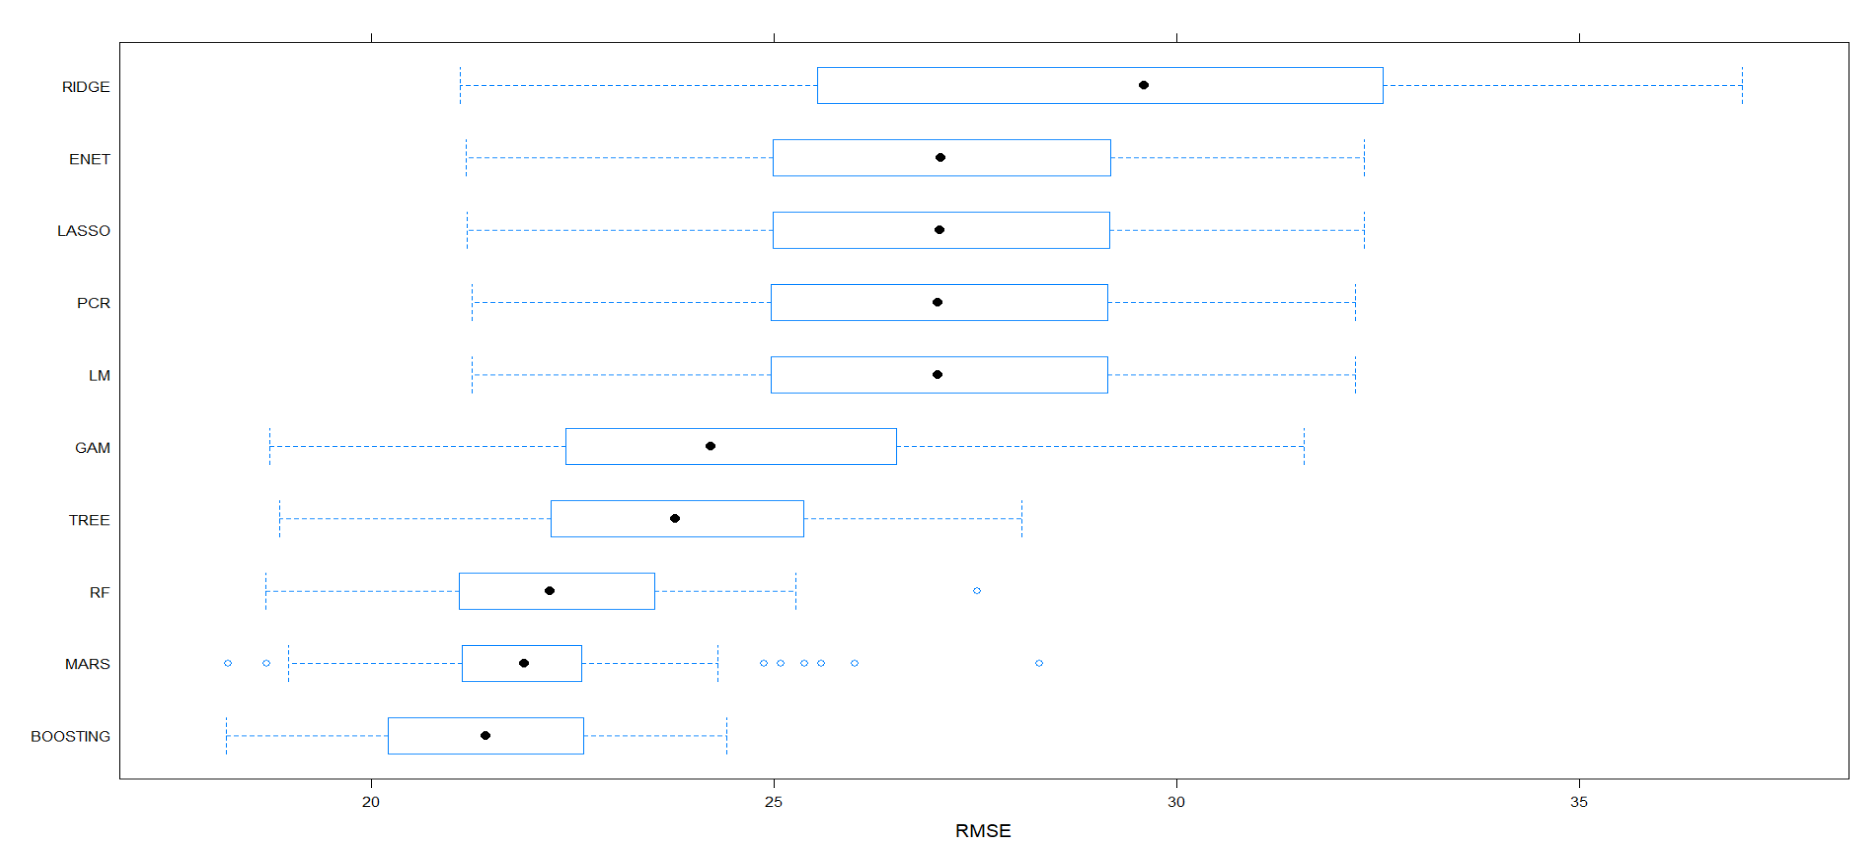
\includegraphics[width=0.9\linewidth,height=0.7\textheight]{primary_analysis_plot/resample_plot} \end{center}
\begin{center}
Figure 3. the Distribution of RMSE of the eleven models (regression)
\end{center}

From Figure 3, the boosted tree model have the smallest RMSE.

\begin{center}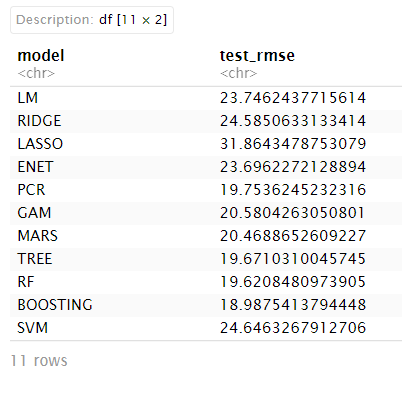
\includegraphics[width=0.9\linewidth,height=0.7\textheight]{primary_analysis_plot/test_rmse} \end{center}
\begin{center}
Table 1. RMSE of the eleven models for prediction (regression)
\end{center}

From Table 1, the boosted tree model had the smallest RMSE which is
about 18.988.

\begin{center}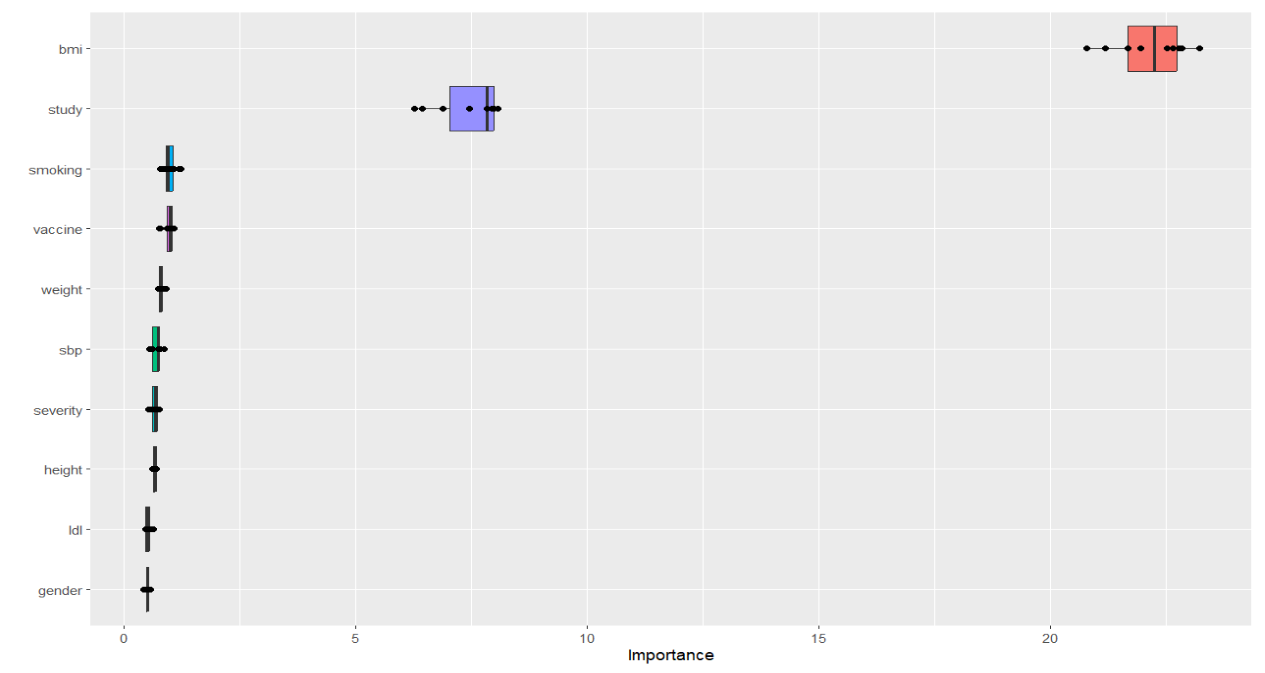
\includegraphics[width=0.9\linewidth,height=0.7\textheight]{primary_analysis_plot/variable_selection} \end{center}
\begin{center}
Figure 4. the Variable Importance Plot (regression)
\end{center}

As for classification, shown in Figure 5, the boosted tree model has the
smallest mean and median RMSE, so we selected it as the best model, same
as regression, to predict the binary value of time to recovery from
COVID-19. We also estimated the performance of the final model with the
test data. Shown in Figure 6, the R-Squared of the boosted tree model is
70.81\%, revealing that around 70\% of the variability observed in the
outcome is explained by this model. And the most important variable in
the final model for classification is bmi.

\begin{center}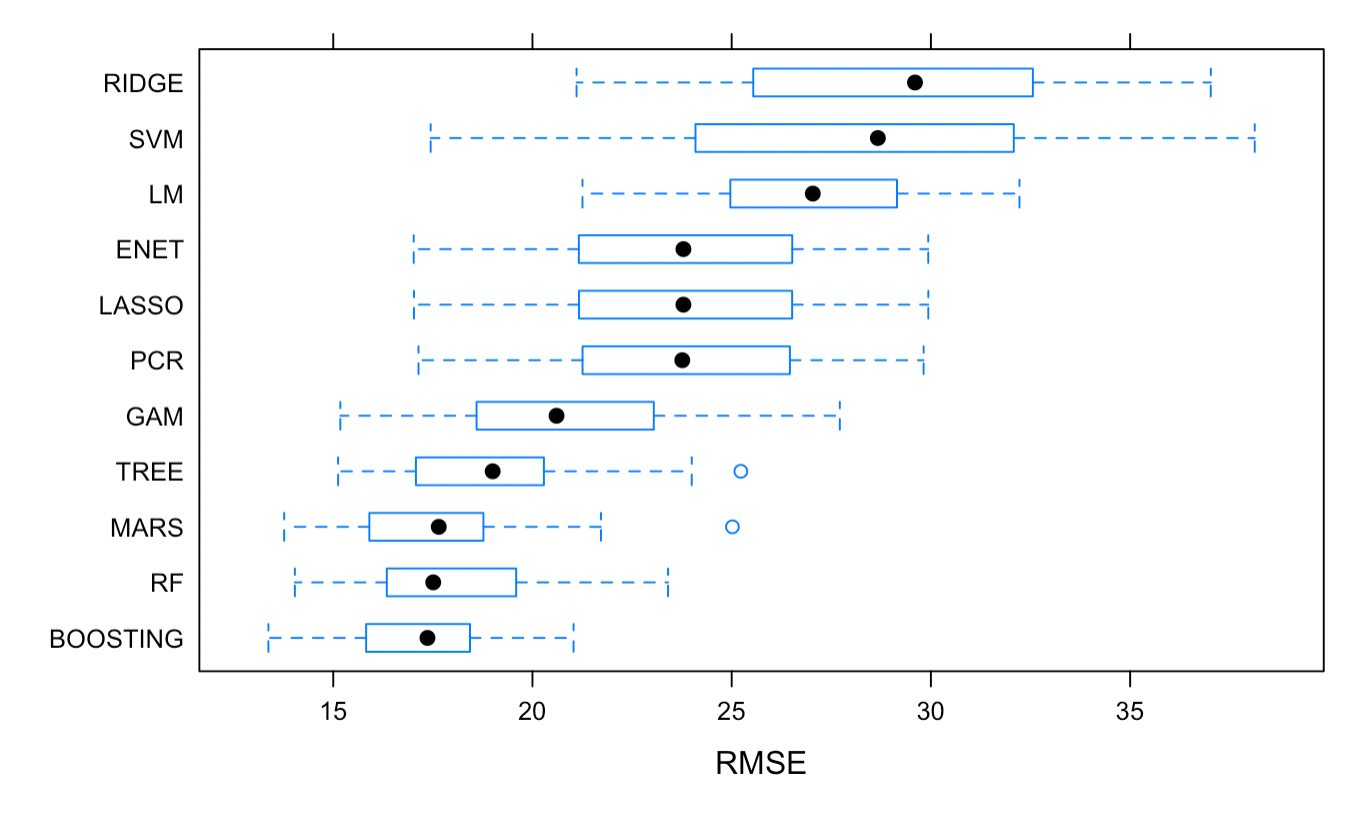
\includegraphics[width=0.9\linewidth,height=0.7\textheight]{secondary_analysis_plot/resample} \end{center}
\begin{center}
Figure 5. Distribution of RMSE of the eleven models (classification)
\end{center}

From Figure 5, the boosted tree model had the smallest RMSE, so it
should be selected as the final model with the best performance.

\begin{center}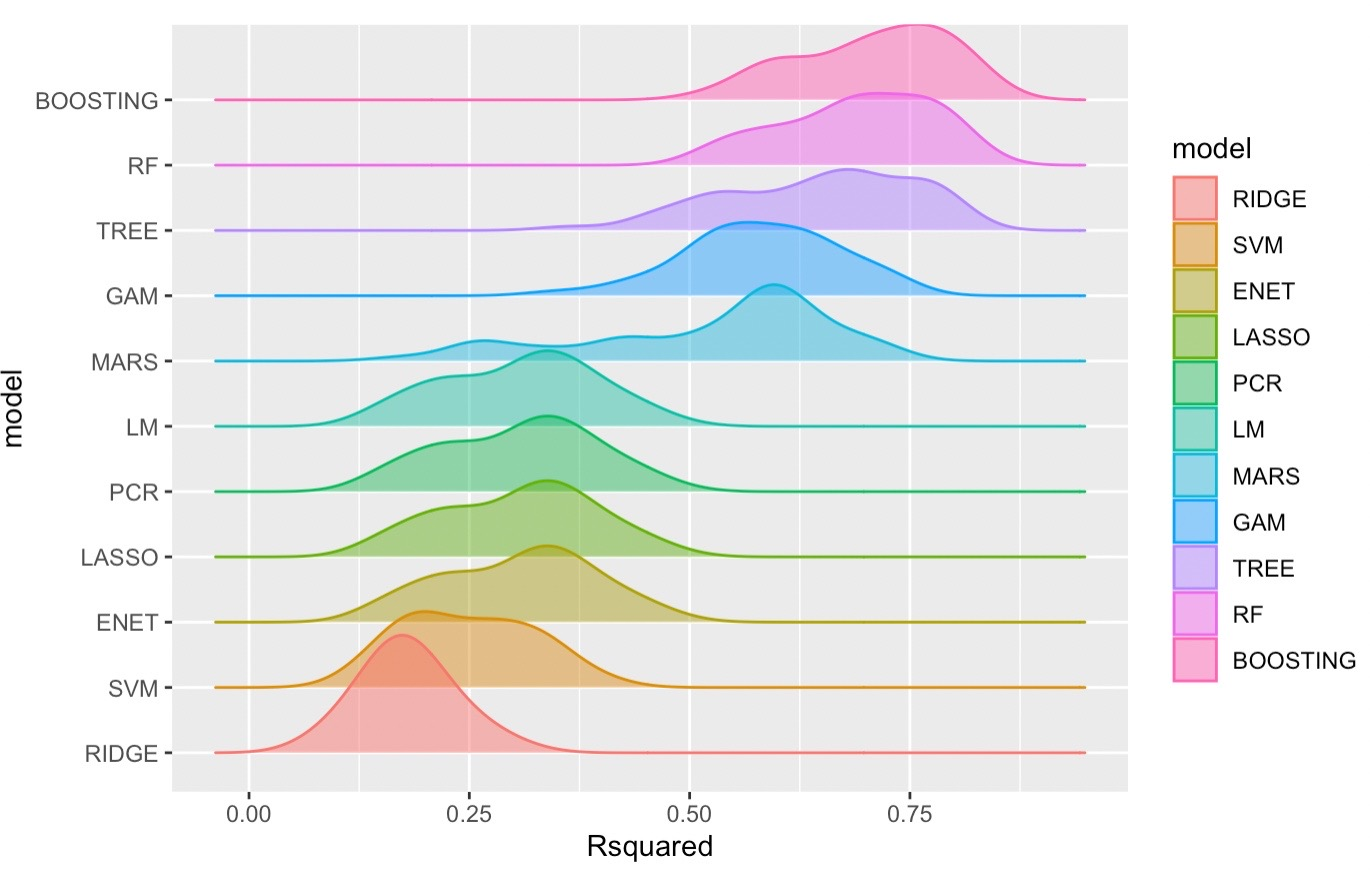
\includegraphics[width=0.9\linewidth,height=0.7\textheight]{secondary_analysis_plot/accuracy} \end{center}
\begin{center}
Figure 6. Prediction accuracy of the eleven models (classification)
\end{center}

Theoretically, the regression model can still fit binary data, but it
will produce wrong fitting results. To illustrate this point, in
Figure.6 we compare the accuracy of the classification model with the
regression models used in the primary analysis. The results show that
Boosting, RF, TREE, GAM and MARS have higher accuracy, indicating a
better fit. Besides, according to Figure.6, the boosted tree model have
the largest R squared value, so it should be chosen as the final model
with the best performance.

\hypertarget{discussion}{%
\section{Discussion}\label{discussion}}

From the EDA above, we observed high correlation between bmi and
recovery time, which supports our finding in primary analysis that bmi
is a significant variable to predict recovery time in the final model.
However, study type, as the second most important predictor of the final
model, has no significant correlation with recovery time in EDA. We
presumed that there might be interaction among study and some other
variables, which requires further research and analysis in the future.

\hypertarget{conclusion}{%
\section{Conclusion}\label{conclusion}}

To identify important risk factors for longer recovery time and gain a
better understanding of the predictors of recovery time from COVID-19,
we compared eleven models both for regression and classification
respectively with a dataset of 3595 observations and 14 predictors.
Among them, the boosted tree models show the greatest performance on
predicting time to recovery from COVID-19, with RMSE 18.99 for
regression and R-Squared 70.81\% for classification.

\newpage

\hypertarget{appendix}{%
\section{Appendix}\label{appendix}}

\hypertarget{tables-and-figures-for-regression}{%
\subsection{Tables and figures for
regression}\label{tables-and-figures-for-regression}}

\begin{center}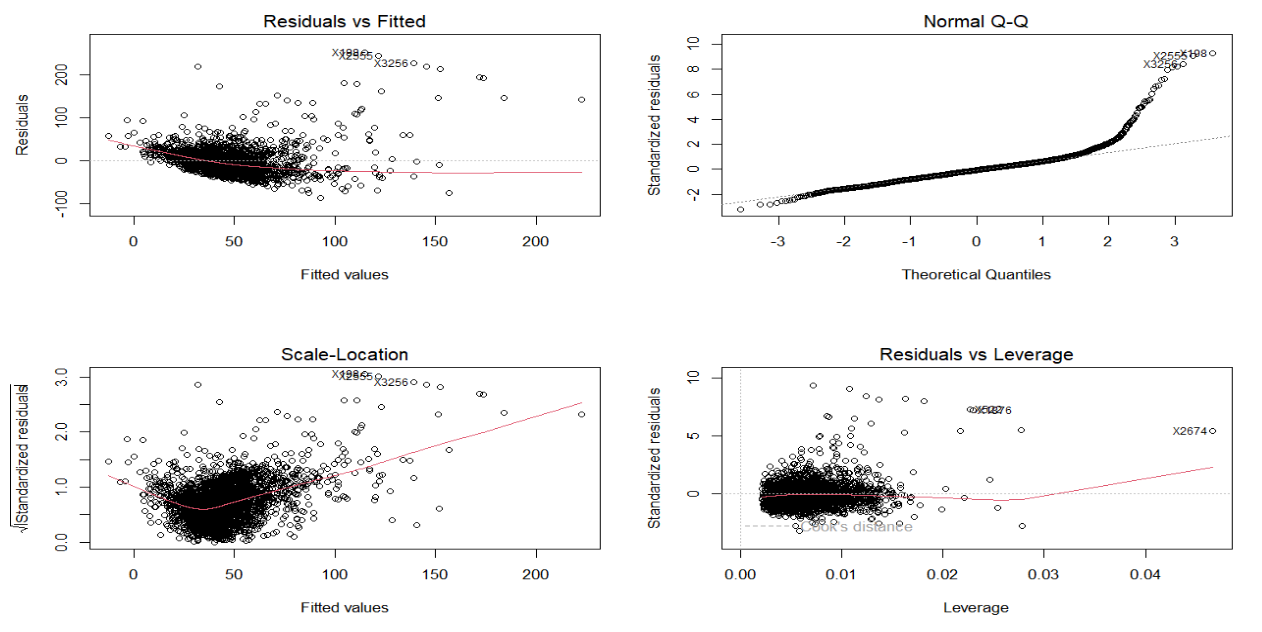
\includegraphics[width=0.9\linewidth,height=0.7\textheight]{primary_analysis_plot/linear_plots} \end{center}
\begin{center}
Appendix I. Linear model
\end{center}

\begin{center}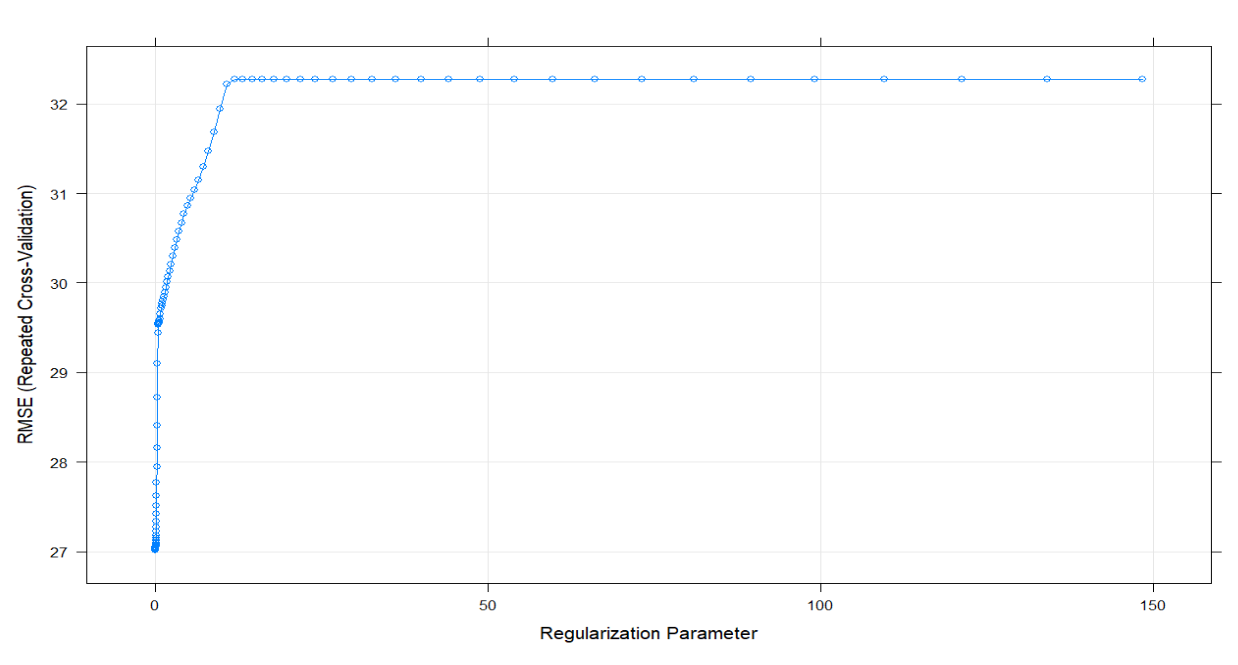
\includegraphics[width=0.9\linewidth,height=0.7\textheight]{primary_analysis_plot/lasso_plot} \end{center}
\begin{center}
Appendix II. Lasso
\end{center}

\begin{center}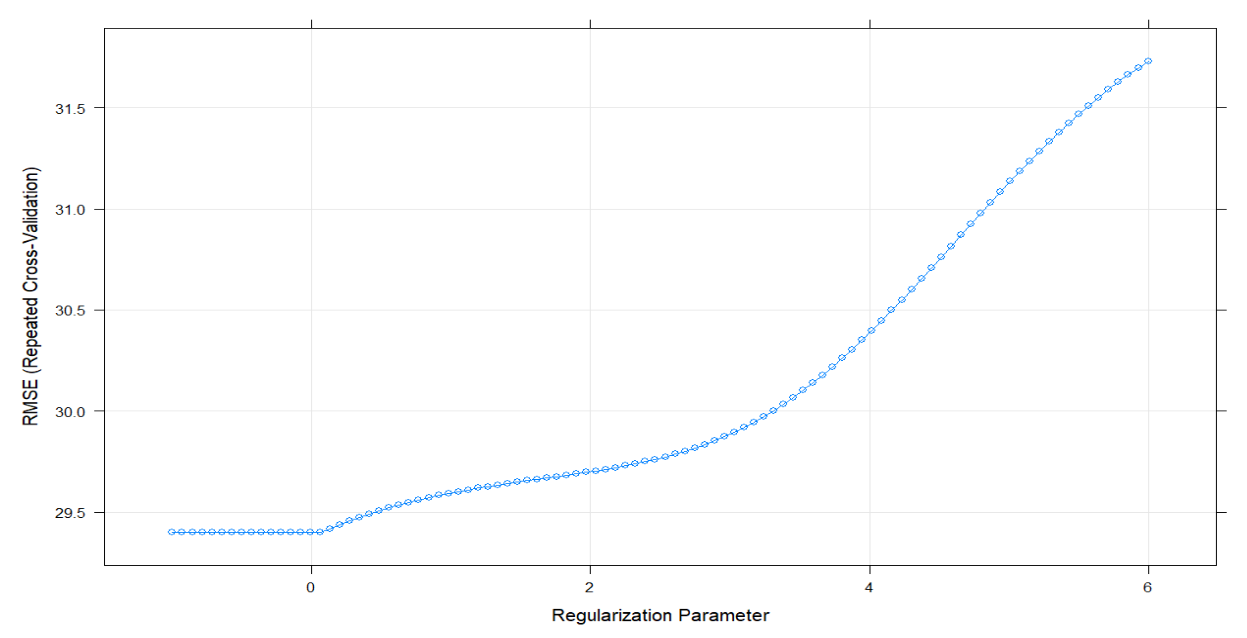
\includegraphics[width=0.9\linewidth,height=0.7\textheight]{primary_analysis_plot/ridge_plot} \end{center}
\begin{center}
Appendix III. Ridge
\end{center}

\begin{center}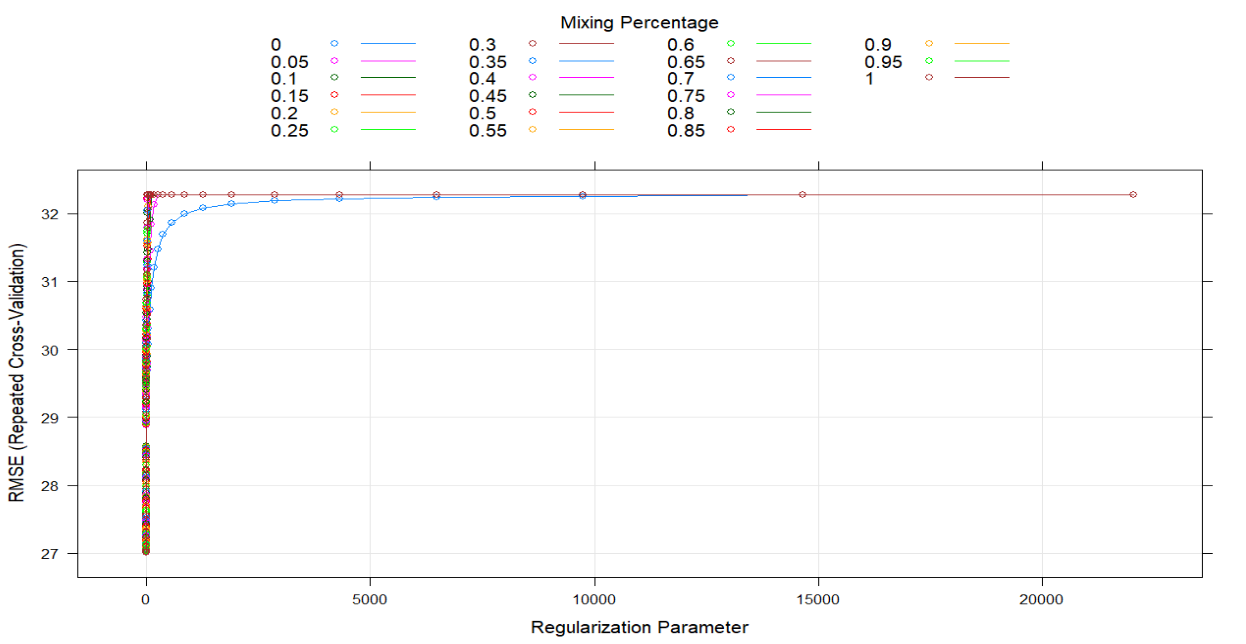
\includegraphics[width=0.9\linewidth,height=0.7\textheight]{primary_analysis_plot/elastic_net_plot} \end{center}
\begin{center}
Appendix IV. Elastic net
\end{center}

\begin{center}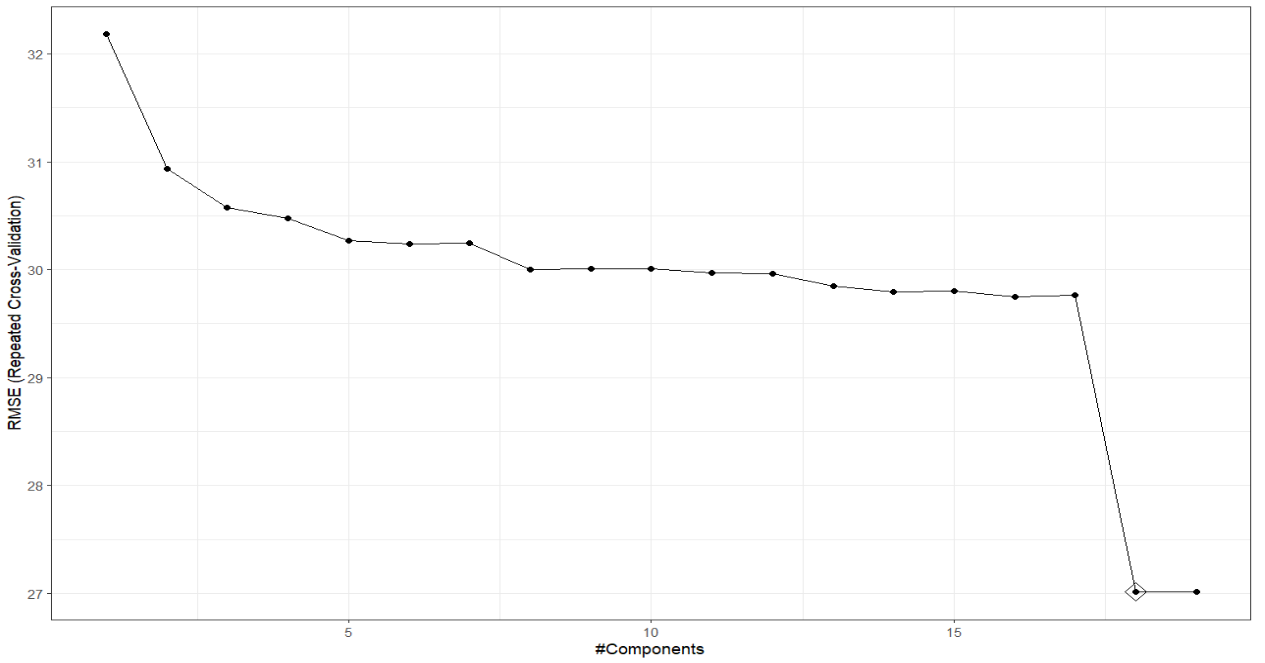
\includegraphics[width=0.9\linewidth,height=0.7\textheight]{primary_analysis_plot/pcr_plot} \end{center}
\begin{center}
Appendix V. PCR
\end{center}

\begin{center}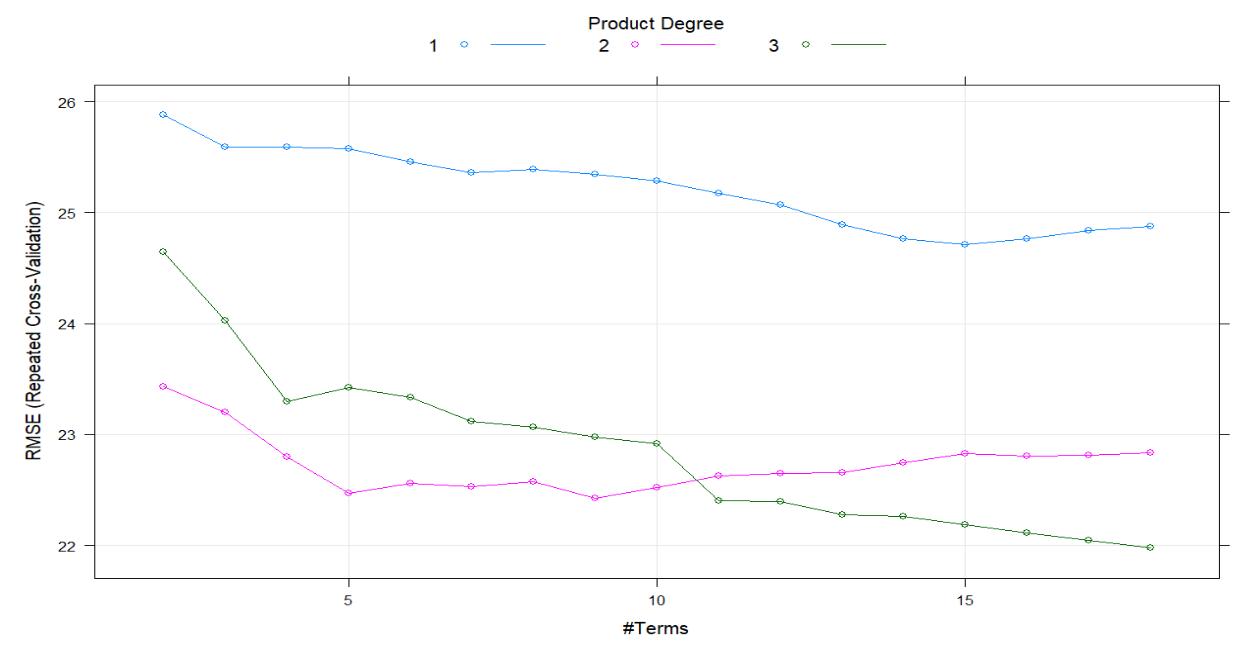
\includegraphics[width=0.9\linewidth,height=0.7\textheight]{primary_analysis_plot/mars_plot} \end{center}
\begin{center}
Appendix VI. MARS
\end{center}

\begin{center}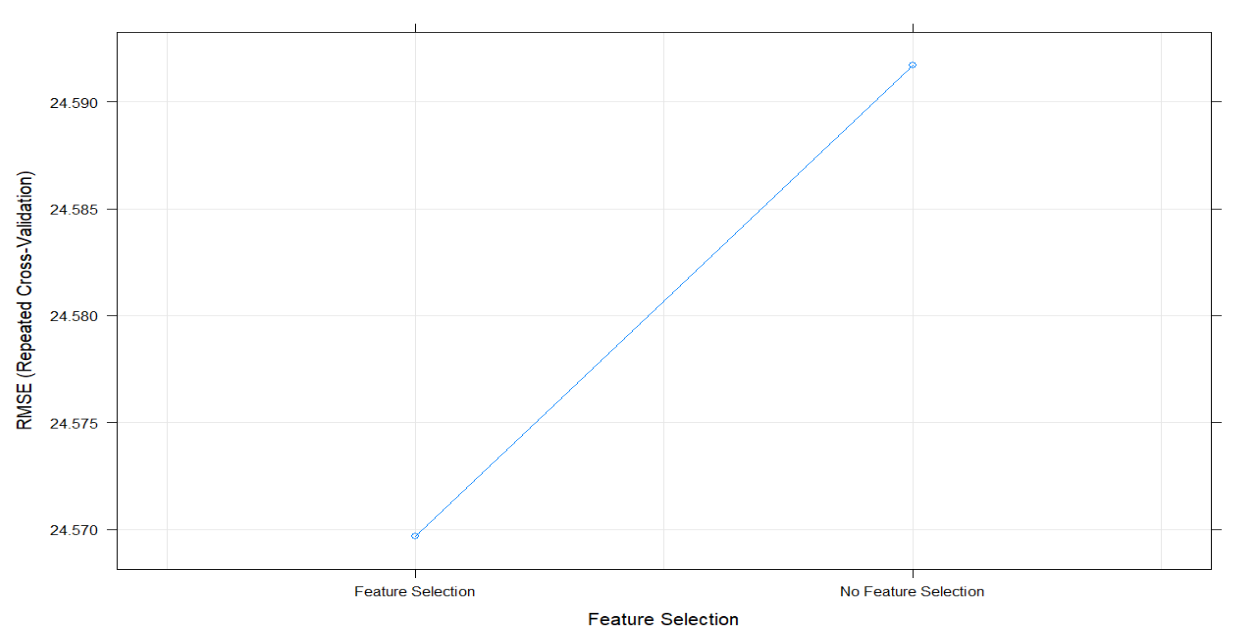
\includegraphics[width=0.9\linewidth,height=0.7\textheight]{primary_analysis_plot/gam_plot} \end{center}
\begin{center}
Appendix VII. GAM
\end{center}

\begin{center}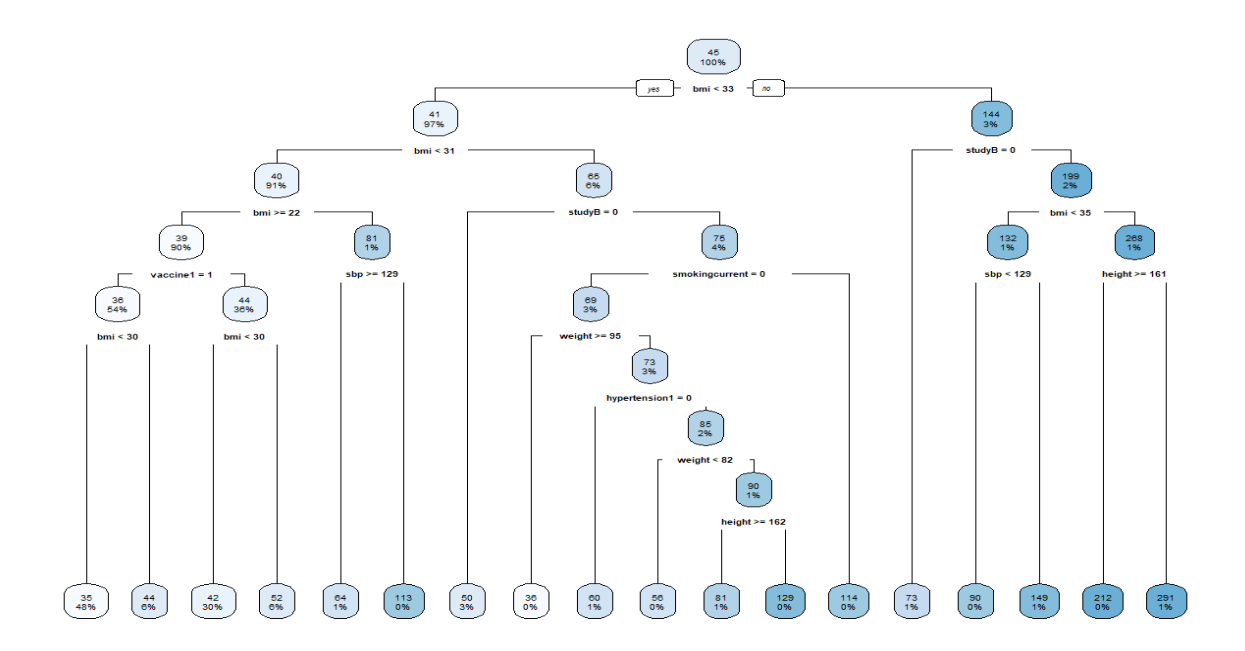
\includegraphics[width=0.9\linewidth,height=0.7\textheight]{primary_analysis_plot/tree_plot_2} \end{center}
\begin{center}
Appendix VIII. Regression tree
\end{center}

\begin{center}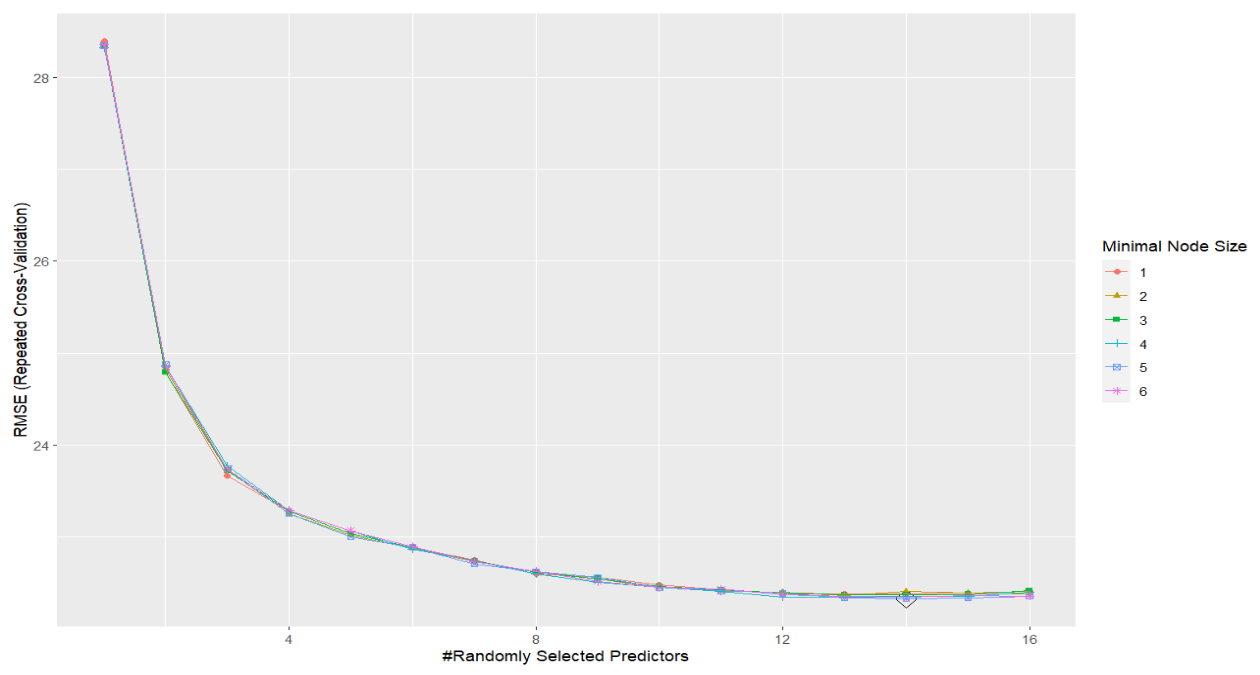
\includegraphics[width=0.9\linewidth,height=0.7\textheight]{primary_analysis_plot/rf_plot} \end{center}
\begin{center}
Appendix VIIII. Bagging
\end{center}

\begin{center}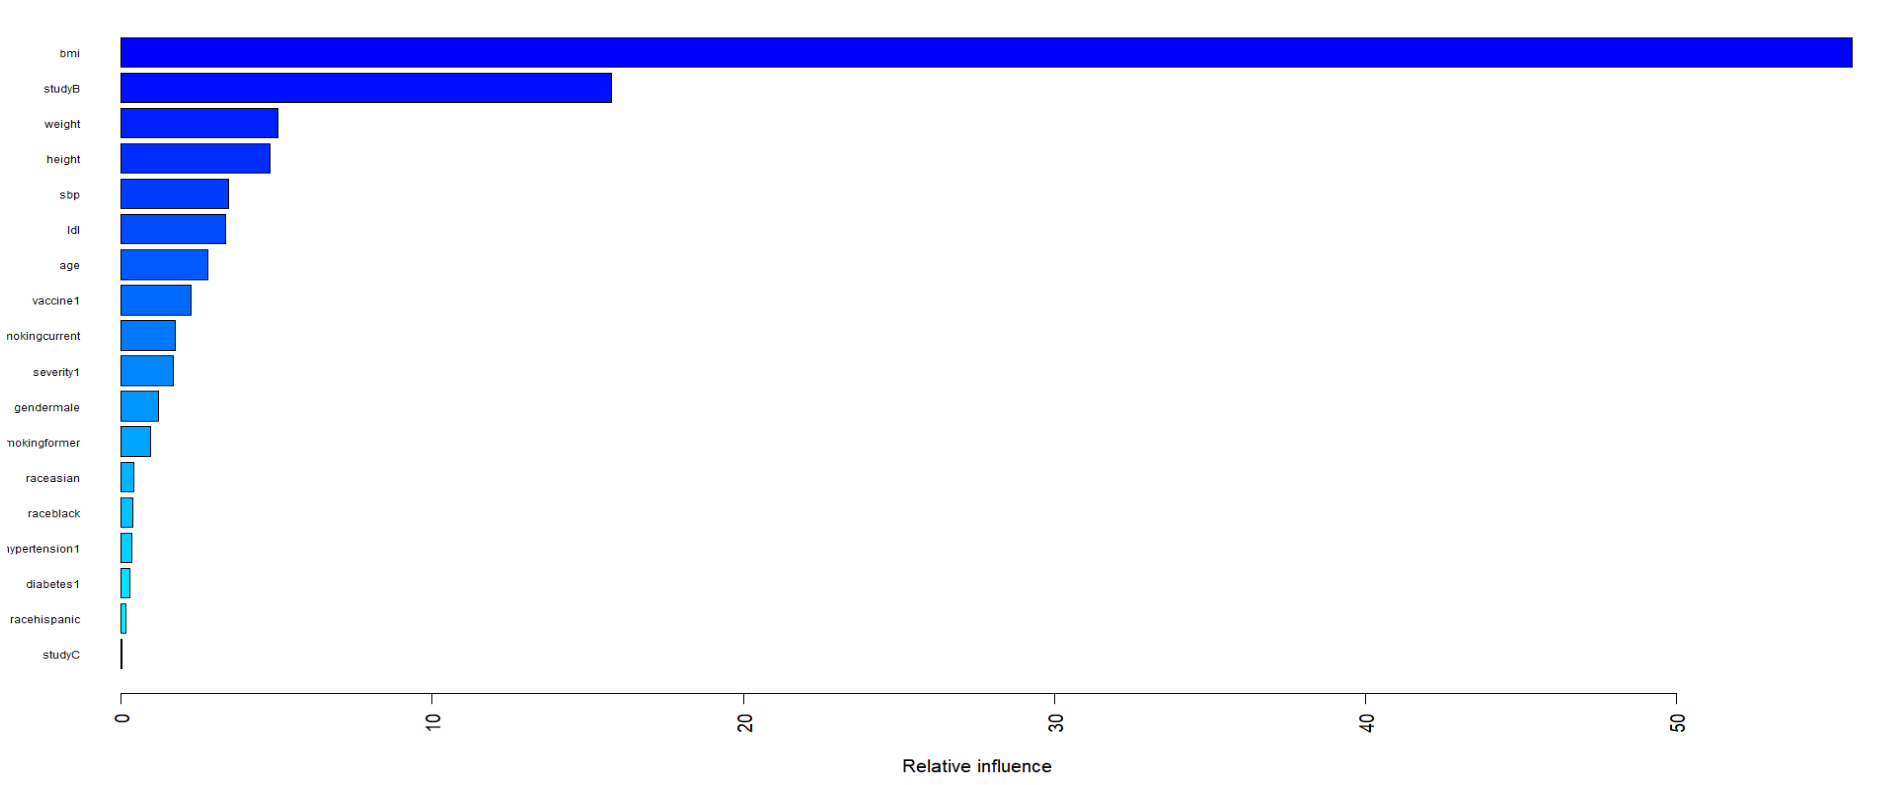
\includegraphics[width=0.9\linewidth,height=0.7\textheight]{primary_analysis_plot/boosting_plot} \end{center}
\begin{center}
Appendix X. Boosted tree model
\end{center}

\begin{center}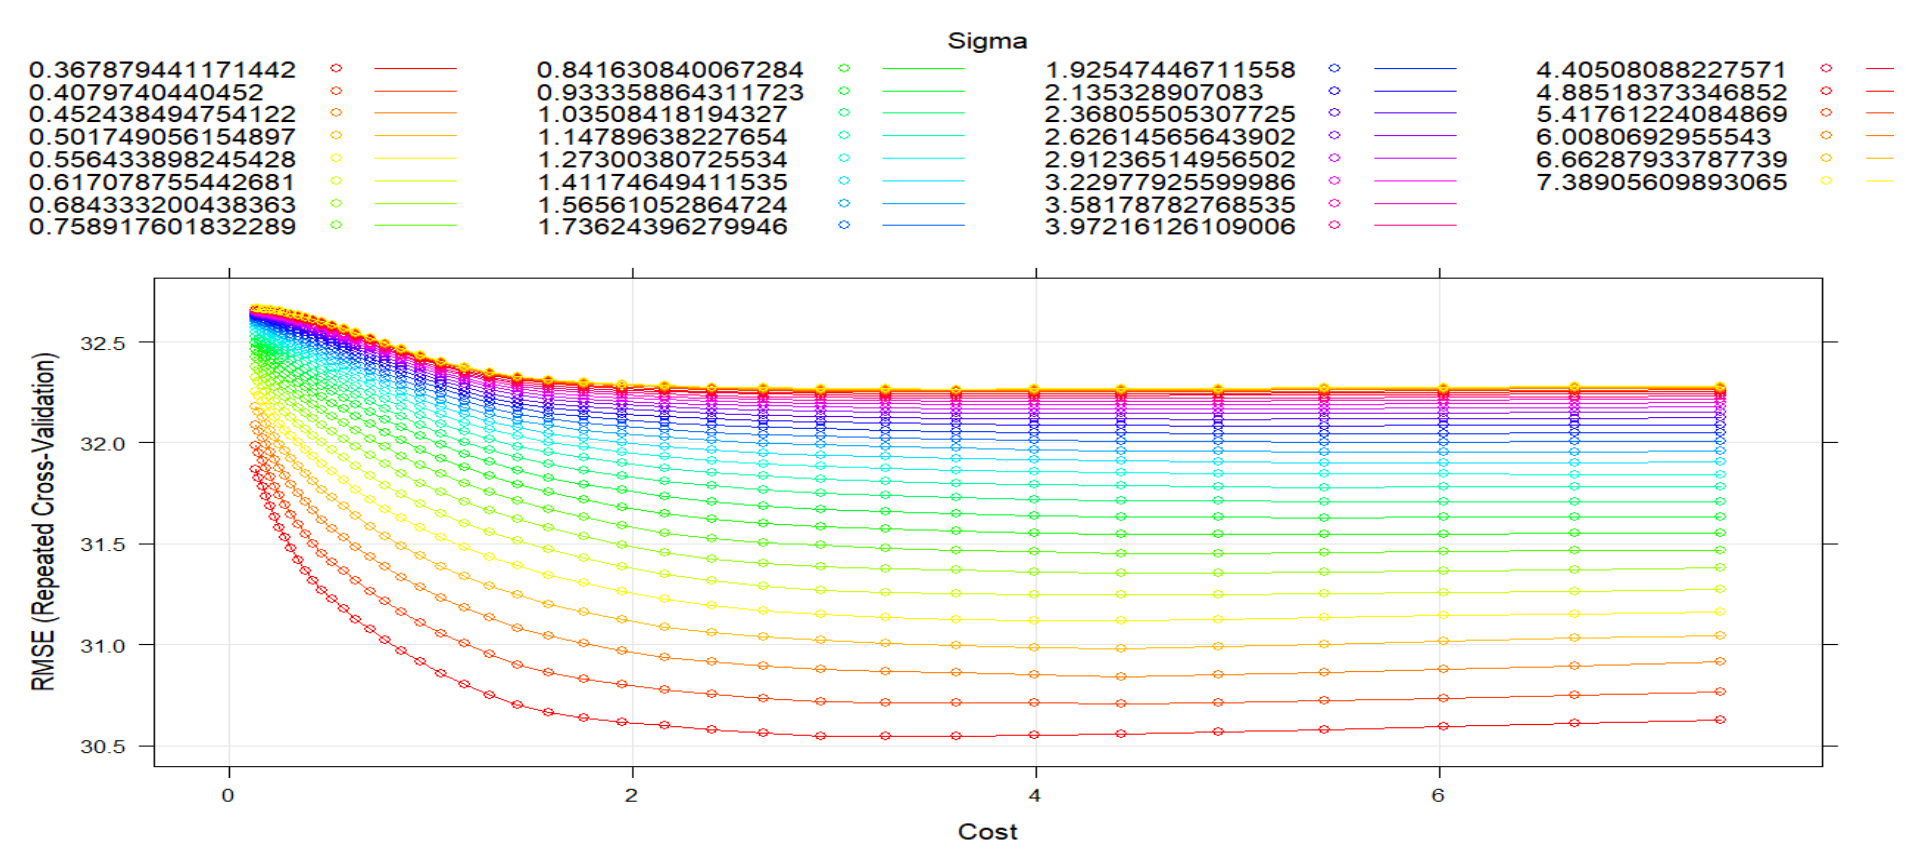
\includegraphics[width=0.9\linewidth,height=0.7\textheight]{primary_analysis_plot/smv_plot} \end{center}
\begin{center}
Appendix XI. SVM
\end{center}

\hypertarget{tables-and-figures-for-classification}{%
\subsection{Tables and figures for
classification}\label{tables-and-figures-for-classification}}

\begin{center}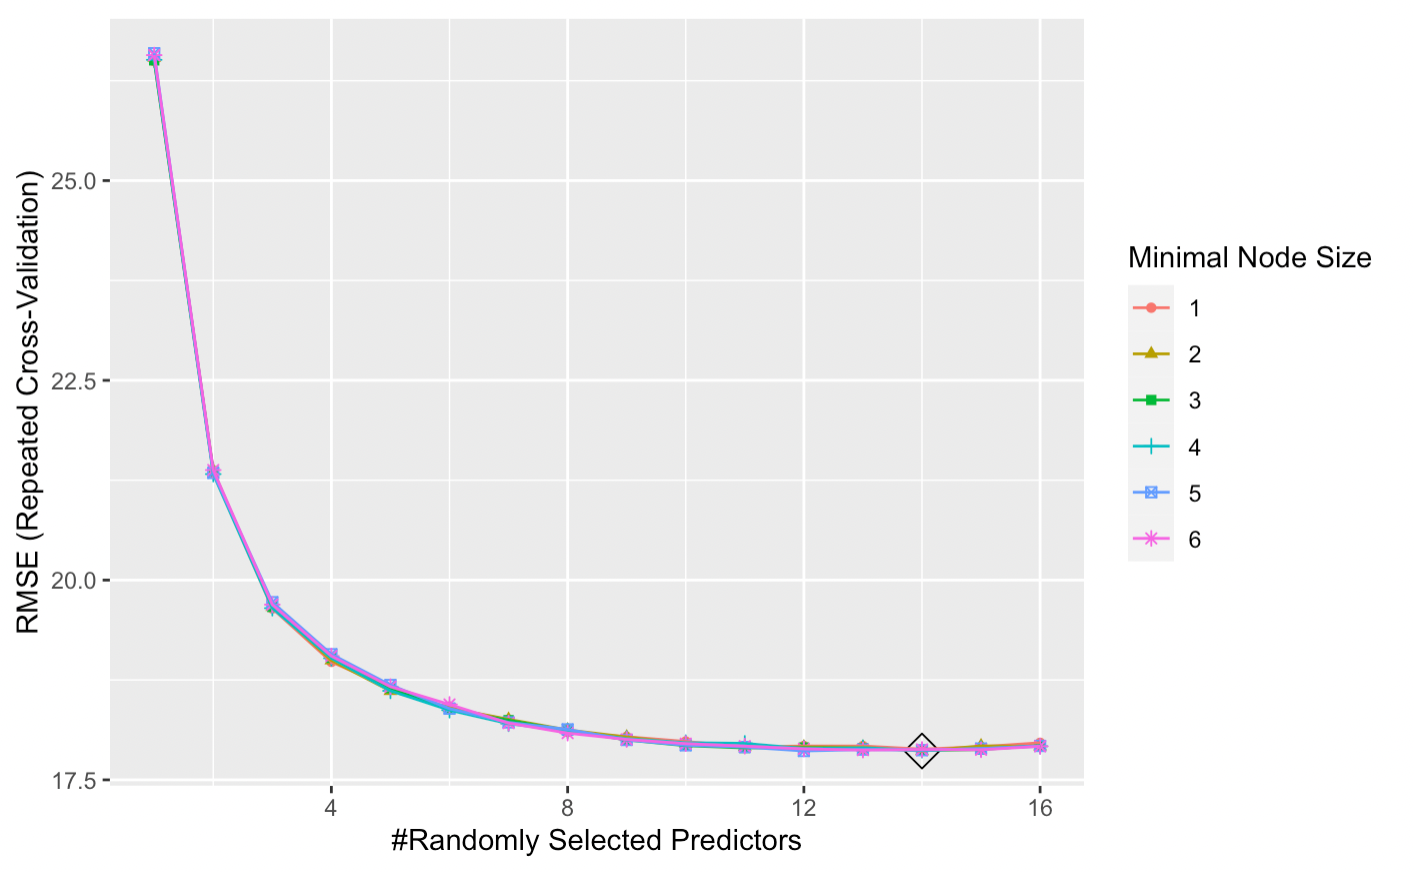
\includegraphics[width=0.9\linewidth,height=0.7\textheight]{secondary_analysis_plot/rf} \end{center}
\begin{center}
Appendix XII. Bagging
\end{center}

\begin{center}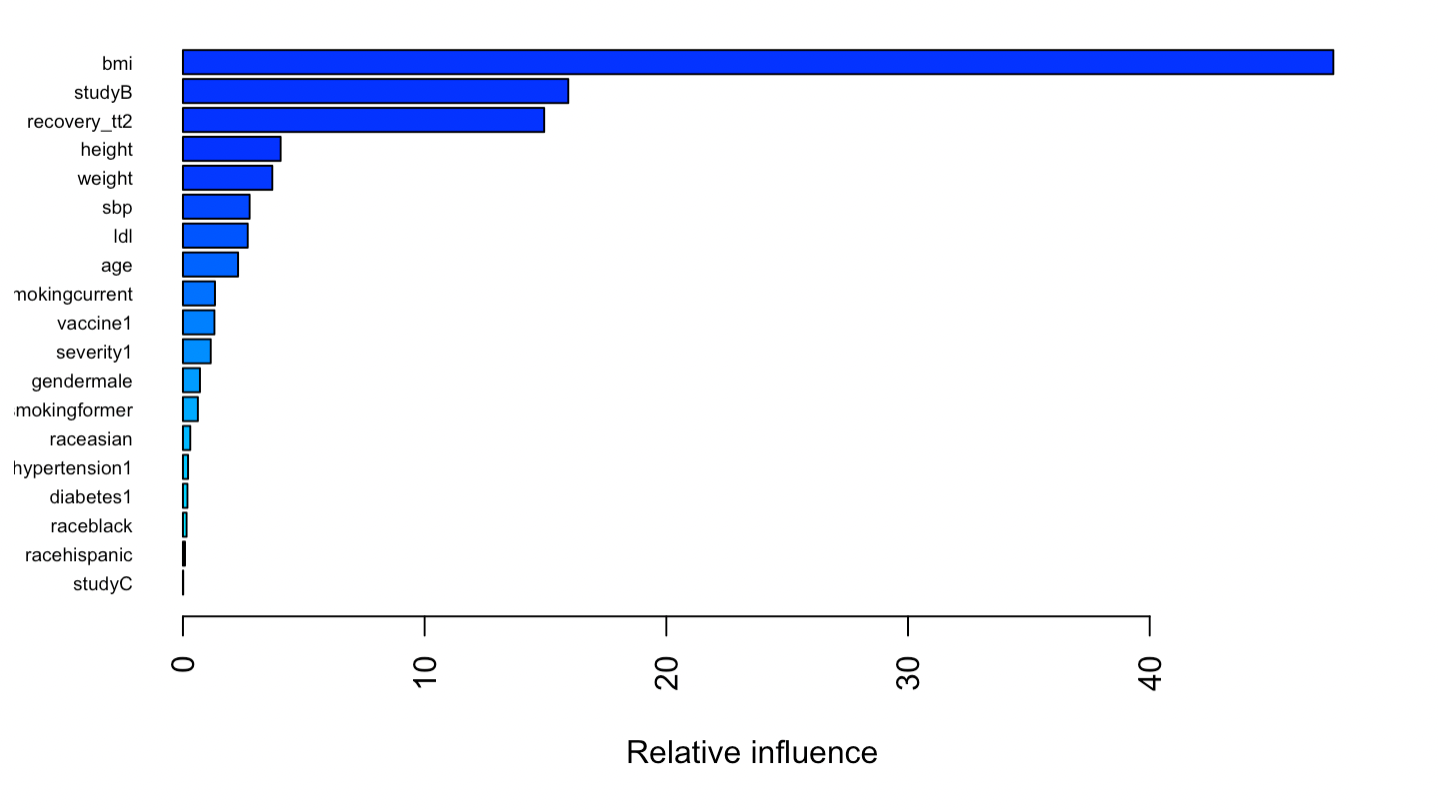
\includegraphics[width=0.9\linewidth,height=0.7\textheight]{secondary_analysis_plot/boosting} \end{center}
\begin{center}
Appendix XIII. Boosting
\end{center}

\begin{center}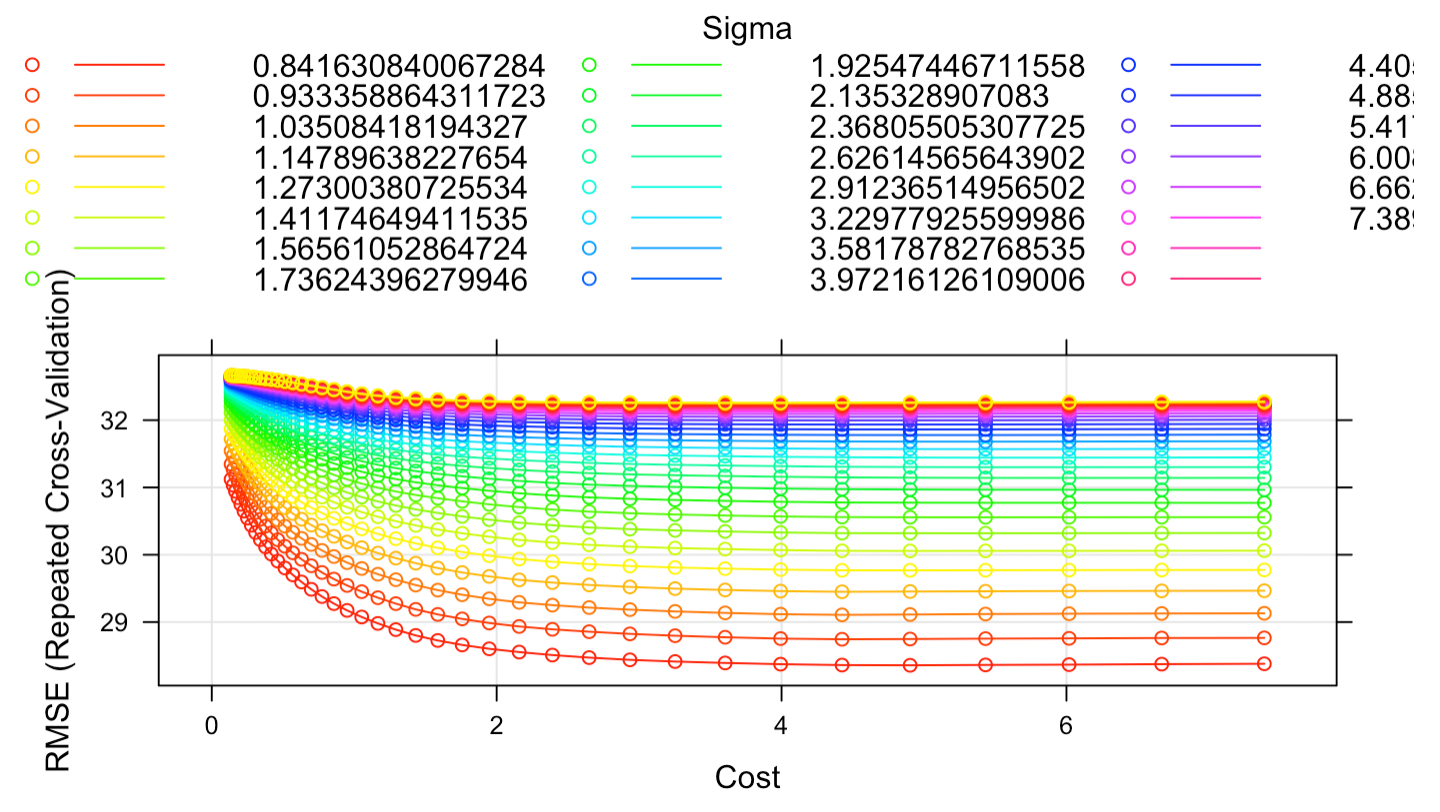
\includegraphics[width=0.9\linewidth,height=0.7\textheight]{secondary_analysis_plot/smv} \end{center}
\begin{center}
Appendix XIV. SVM
\end{center}

\begin{center}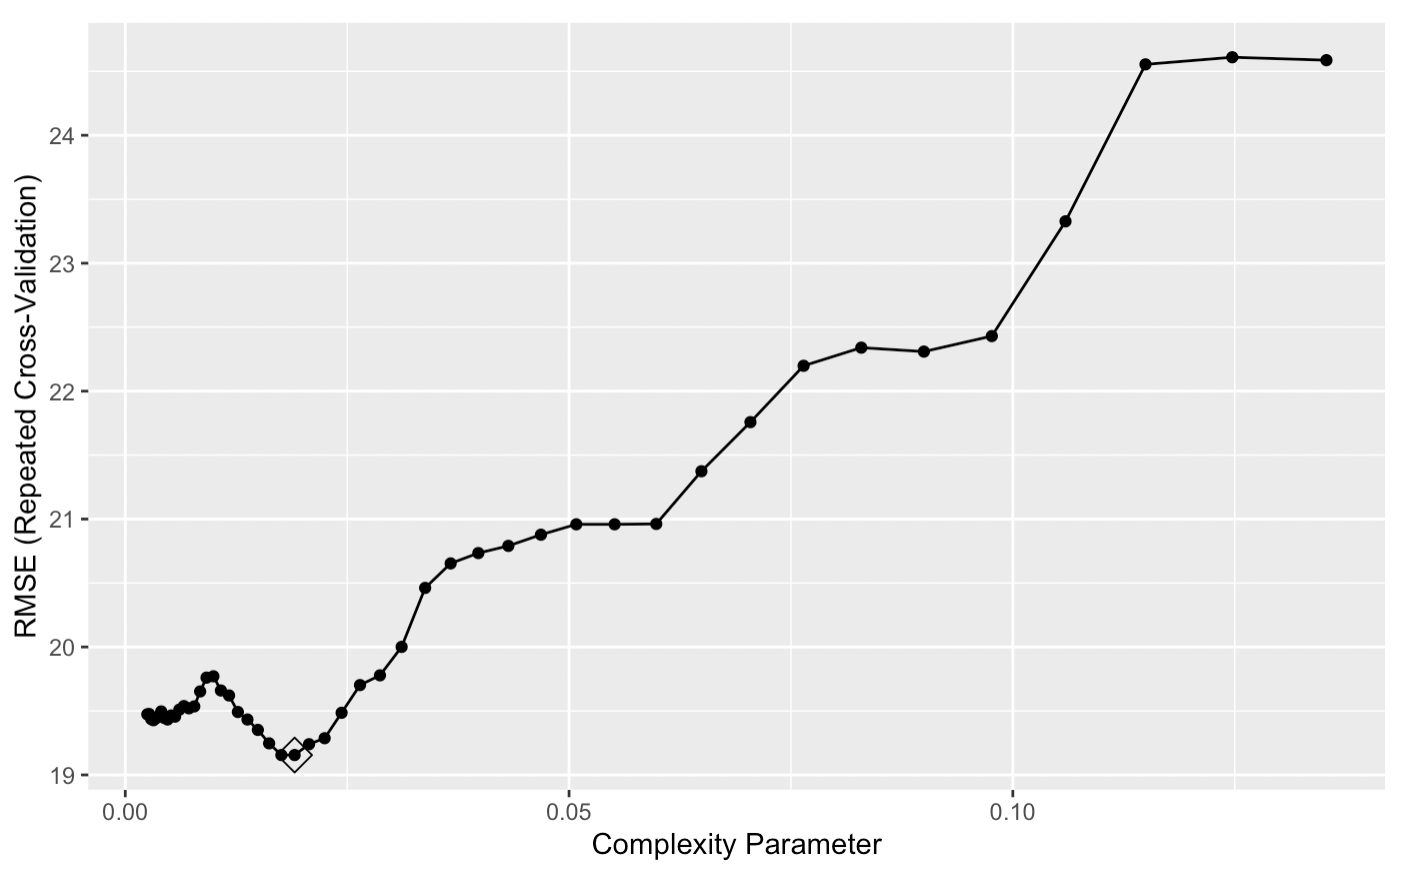
\includegraphics[width=0.9\linewidth,height=0.7\textheight]{secondary_analysis_plot/tree1} \end{center}
\begin{center}
Appendix XV. Classification Tree
\end{center}

\end{document}
